\documentclass[Orbiter User Manual.tex]{subfiles} 
\begin{document}

\section{The solar system neighbourhood}
Orbiter’s playground is our solar system. The basic installation includes its major bodies (the Sun and planets) and a subset of minor bodies (moons and asteroids), providing a variety of mission targets. Planning and executing a trip that is efficient both in duration and fuel consumption offers different challenge levels. Additional objects may be downloaded as add-ons.

\begin{figure}[H]
	\centering
	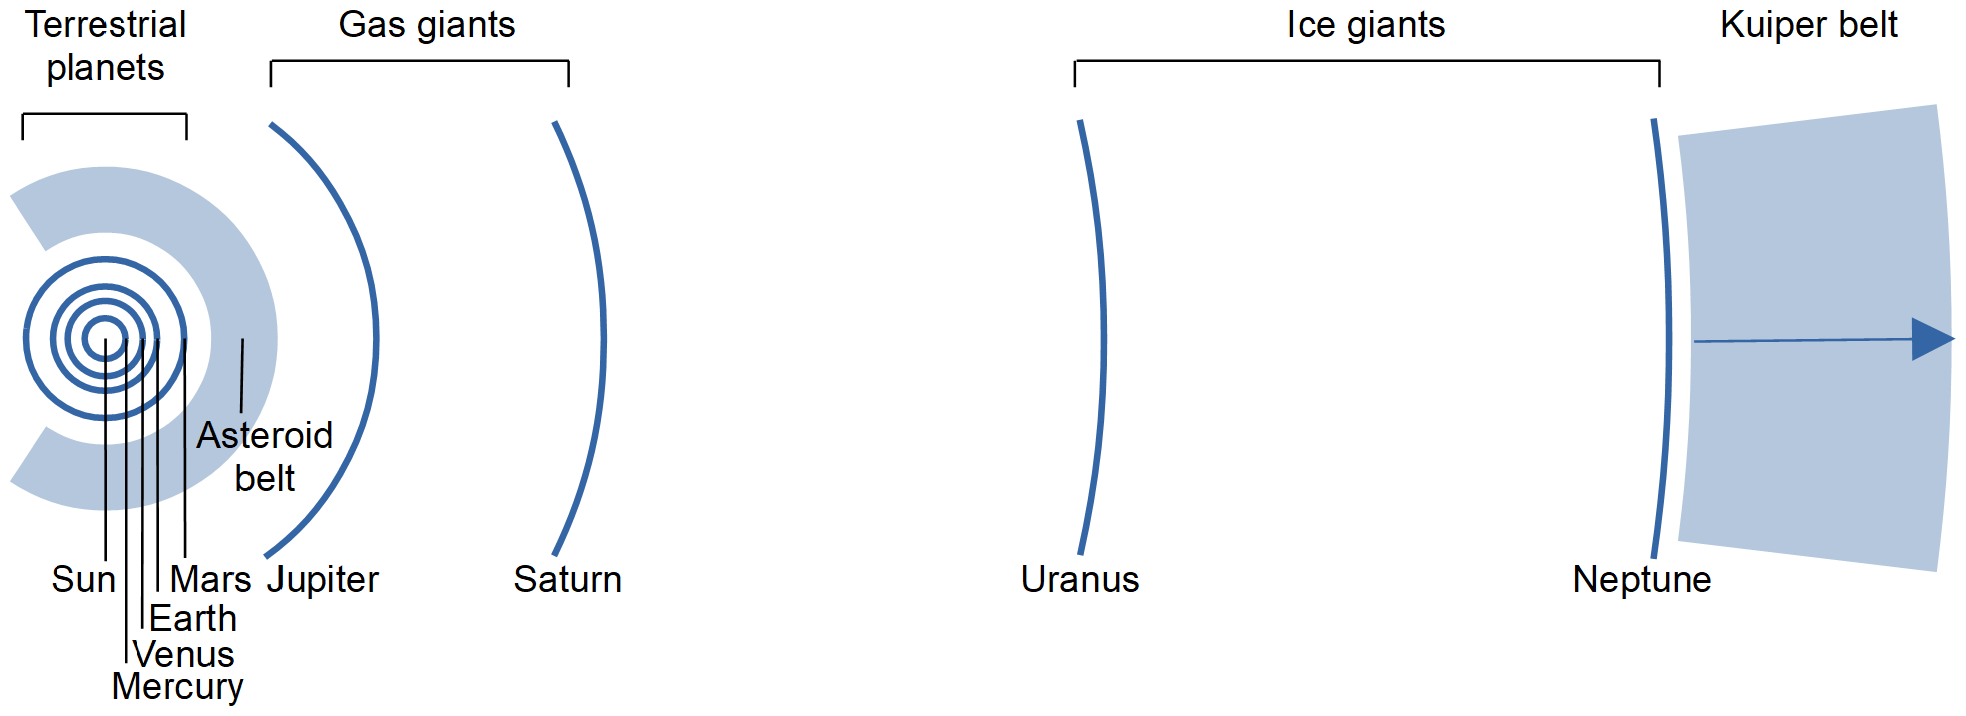
\includegraphics[width=0.99\hsize]{sol.png}
\end{figure}


\subsection{Solar system bodies}

\begin{table}[H]
	\begin{tabularx}{\textwidth}{ |lX| }
	\hline\rule{0pt}{2ex}
	\textbf{Sun} &\\
	\hline\rule{0pt}{2ex}
	\adjustbox{valign=t}{
		\begin{tabular}{ c }
		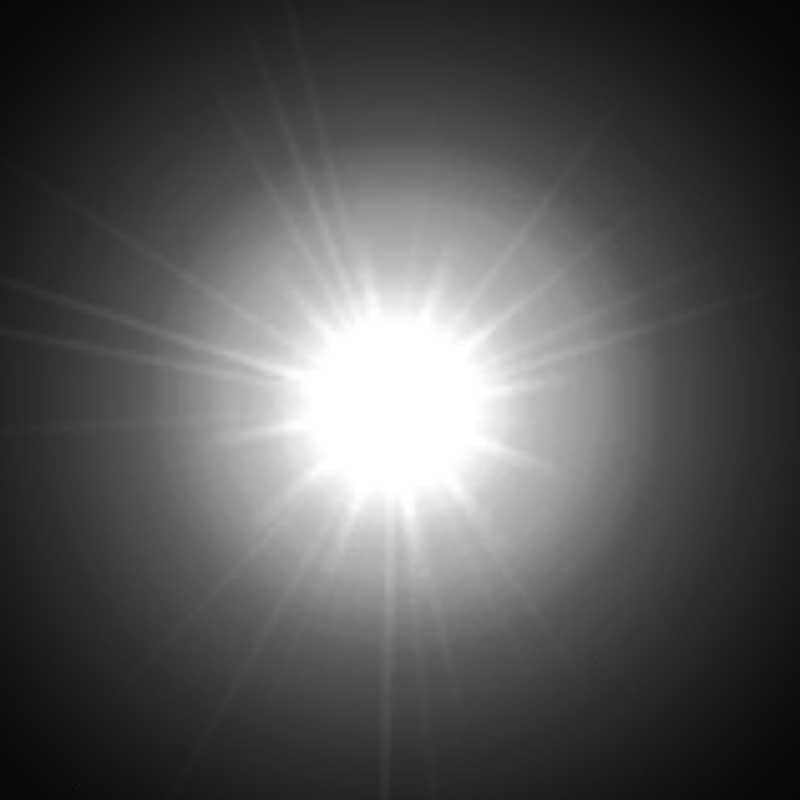
\includegraphics[width=0.6\textwidth, margin=-10pt 1ex -10pt 1ex, valign=m]{solsys_sun.jpg}\\
		\end{tabular}
		}
	& \vfill
	The Sun is a type G2 main sequence star at the centre of our solar system, formed approximately 4.6 billion years ago from a gravitationally collapsing interstellar gas cloud. It comprises nearly the entire mass of the solar system and emits a large amount of electromagnetic energy generated by nuclear fusion in its core. In another 5 billion years the hydrogen fuel will be exhausted and the Sun will expand into a red giant, losing a significant amount of its mass, before the remaining core, a white dwarf, will slowly cool down over trillions of years.\\
	\hline
	\end{tabularx}
\end{table}


\begin{table}[H]
	\begin{tabularx}{\textwidth}{ |lX| }
	\hline\rule{0pt}{2ex}
	\textbf{Mercury} &\\
	\hline\rule{0pt}{2ex}
	\adjustbox{valign=t}{
		\begin{tabular}{ c }
		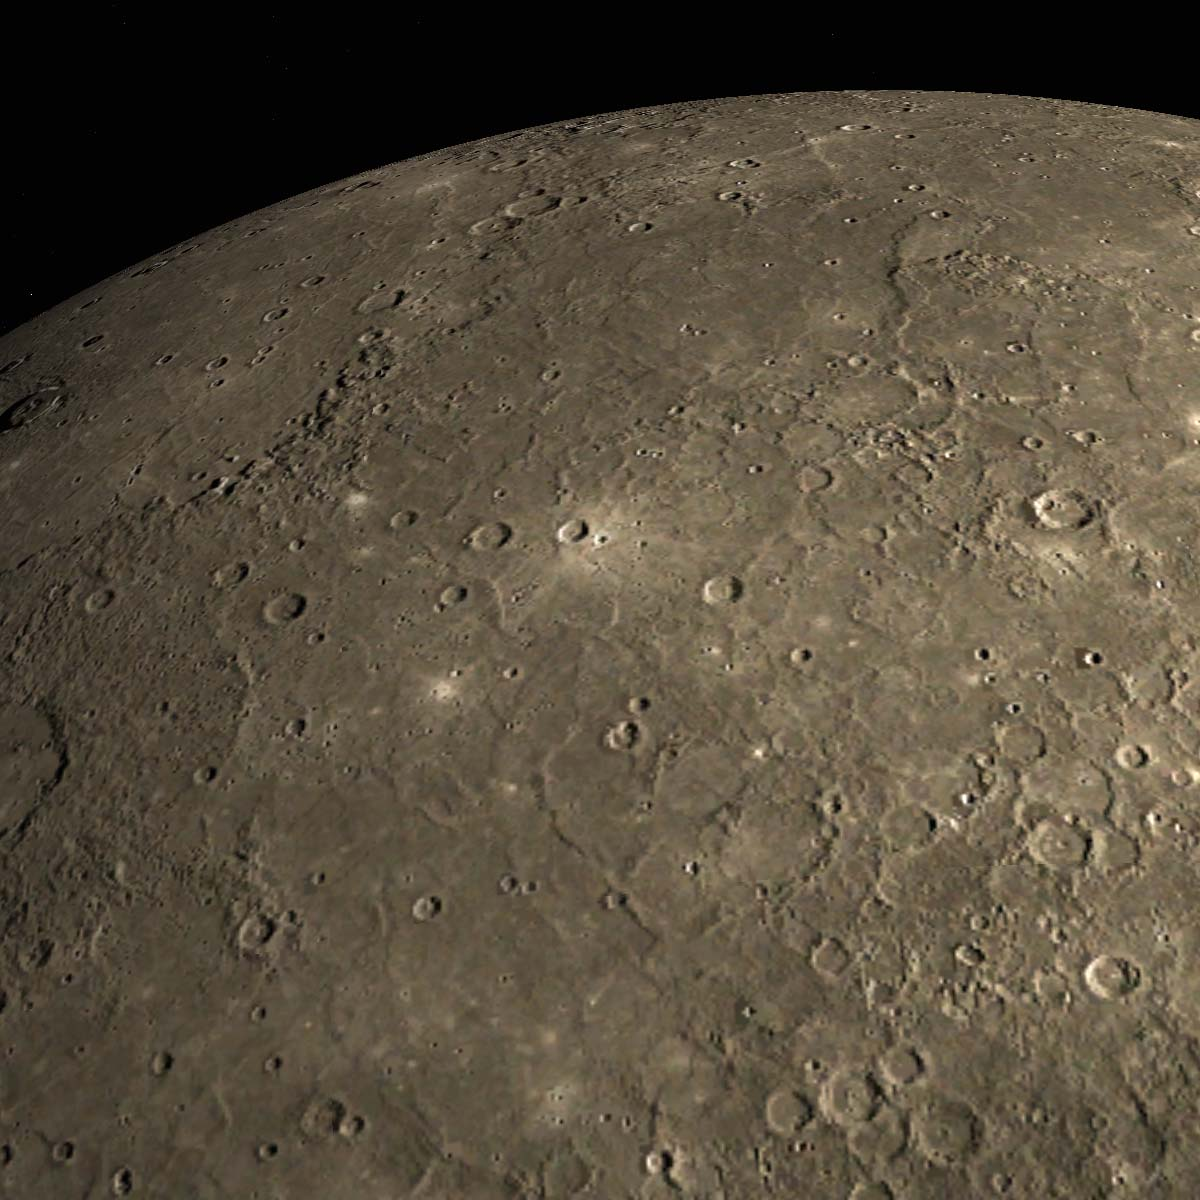
\includegraphics[width=0.6\textwidth, margin=-10pt 1ex -10pt 1ex, valign=m]{solsys_mercury.jpg}\\
		\end{tabular}
		}
	& \vfill
	Mercury is one of the four terrestrial (rocky) inner planets of the solar system. Its orbit is the closest to the Sun and the most eccentric of all planets.\newline
		Mercury has no significant atmosphere, and its slow rotation (it is tidally locked with the Sun in in a 3:2 spin-orbit resonance) results in a large variation between day and night surface temperatures. The surface is heavily cratered and similar in appearance to Earth’s Moon.\newline
		\newline
		\textit{Mercury’s visual representation in Orbiter is based on images from the Messenger mission.}\\
	\hline
	\end{tabularx}
\end{table}


\begin{table}[H]
	\begin{tabularx}{\textwidth}{ |lX| }
	\hline\rule{0pt}{2ex}
	\textbf{Venus} &\\
	\hline\rule{0pt}{2ex}
	\adjustbox{valign=t}{
		\begin{tabular}{ c }
		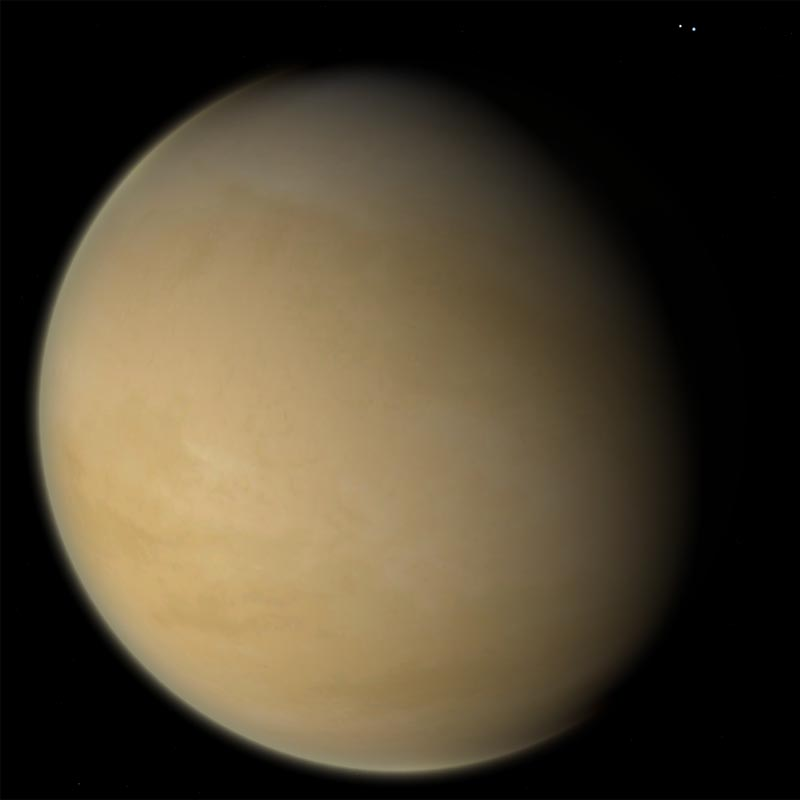
\includegraphics[width=0.6\textwidth, margin=-10pt 1ex -10pt 1ex, valign=m]{solsys_venus.jpg}\\
		\end{tabular}
		}
	& \vfill
	Venus is the second planet from the Sun, and similar in mass and size to Earth. It has a very dense atmosphere of mainly carbon dioxide that completely obscures the surface at visible wavelengths and results in a high albedo. The extreme surface pressure and temperatures pose severe challenges for surface-bound missions.\newline
		\newline
		\textit{In Orbiter, the surface representation of Venus is based on the synthetic aperture radar data from the Magellan mission, while the cloud layer is derived from a map by Björn Jónsson.}\\
	\hline
	\end{tabularx}
\end{table}


\begin{table}[H]
	\begin{tabularx}{\textwidth}{ |lX| }
	\hline\rule{0pt}{2ex}
	\textbf{Earth} &\\
	\hline\rule{0pt}{2ex}
	\adjustbox{valign=t}{
		\begin{tabular}{ c }
		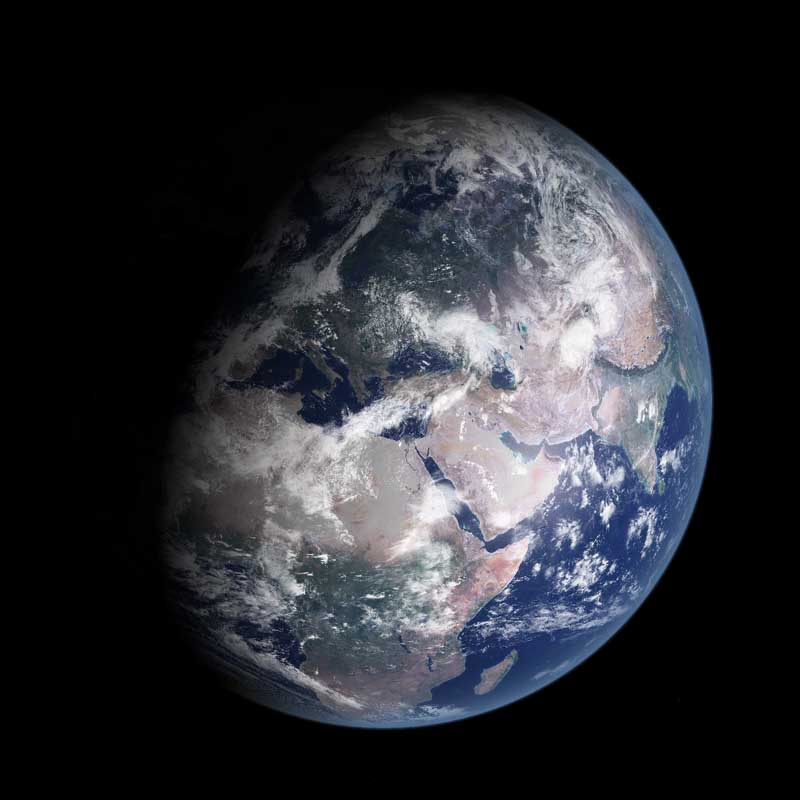
\includegraphics[width=0.6\textwidth, margin=-10pt 1ex -10pt 1ex, valign=m]{solsys_earth.jpg}\\
		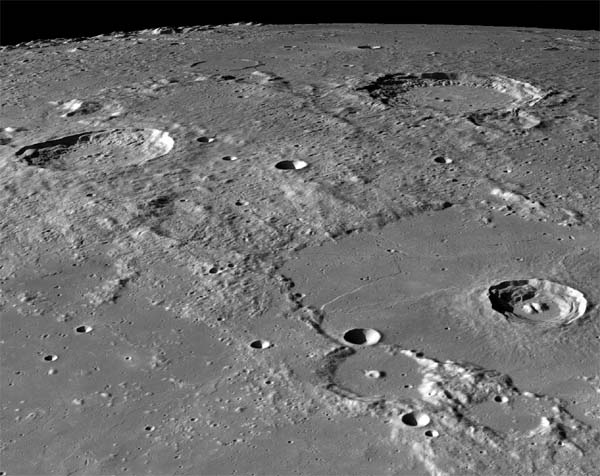
\includegraphics[width=0.6\textwidth, margin=-10pt 1ex -10pt 1ex, valign=m]{solsys_moon.jpg}\\
		\end{tabular}
		}
	& \vfill
	The home planet. Earth is the only place we know to date for life to have evolved. Its distance from the sun, atmospheric conditions and internal heating allow for liquid water to exist in large quantities, forming its oceans. Its atmospheric layer, as well as its magnetic field, protect the surface from harmful radiation. The bio­sphere (the sections of surface, lower atmosphere and oceans containing life) is a self-regulating system whose balance may be threatened by human activity (pollution, release of greenhouse gases).\newline
	The Moon is Earth’s natural satellite. It has no significant atmosphere, and its surface is characterised by impact craters. The Earth-Moon system is unusual in the solar system for the relatively large size of the Moon compared to the planet it orbits, and may have an influence on stabilising Earth’s spin axis.\newline
	\newline
	\textit{In Orbiter, Earth’s surface textures have been custom processed from Landsat-7 ETM orthorectified scenes, augmented by aerial imagery for selected areas. Elevations are from NASA SRTM 90m Digital elevation data. Moon surface textures were generated from LRO LRO-WAC Global Mosaic 100m, elevations from LOLA-GDR/Cylindrical}\\
	\hline
	\end{tabularx}
\end{table}


\begin{table}[H]
	\begin{tabularx}{\textwidth}{ |lX| }
	\hline\rule{0pt}{2ex}
	\textbf{Mars} &\\
	\hline\rule{0pt}{2ex}
	\adjustbox{valign=t}{
		\begin{tabular}{ c }
		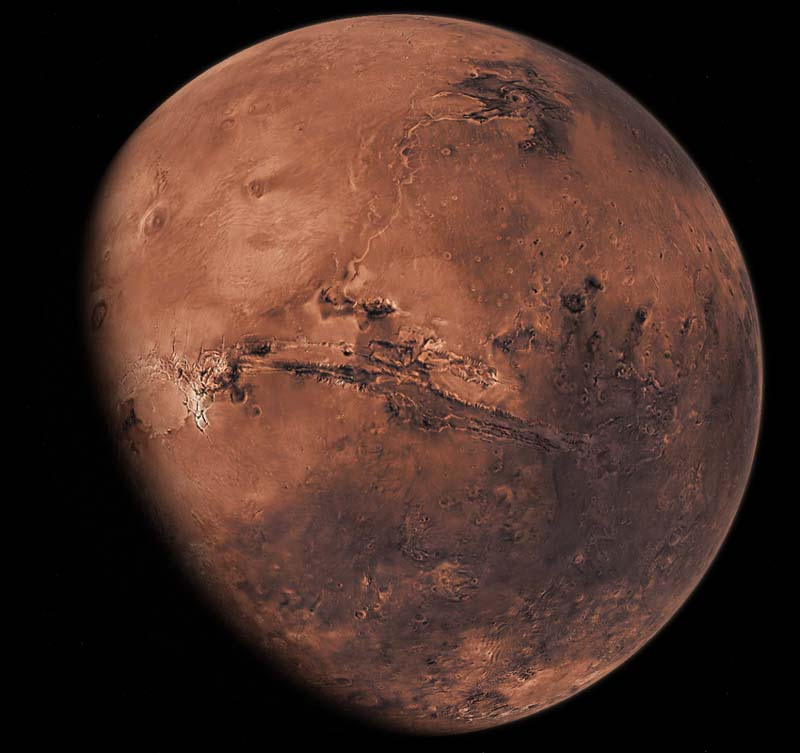
\includegraphics[width=0.6\textwidth, margin=-10pt 1ex -10pt 1ex, valign=m]{solsys_mars.jpg}\\
			\adjustbox{valign=t}{
			\begin{tabular}{ ll }
			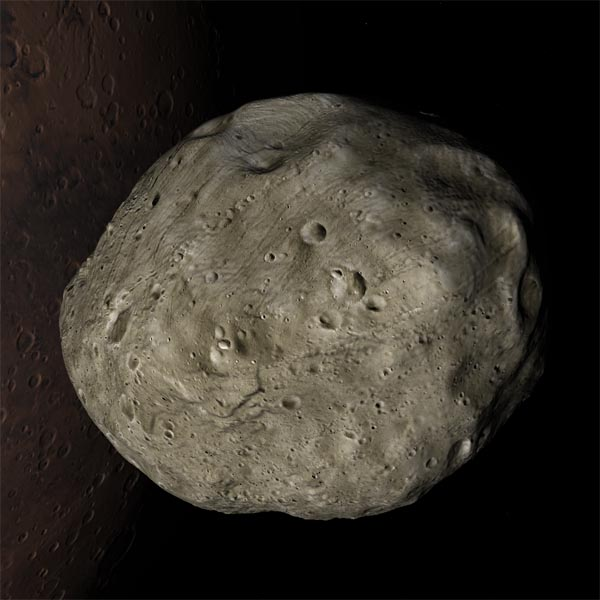
\includegraphics[width=0.285\textwidth, margin=-20pt 1ex 0pt 1ex, valign=m]{solsys_phobos.jpg} &
			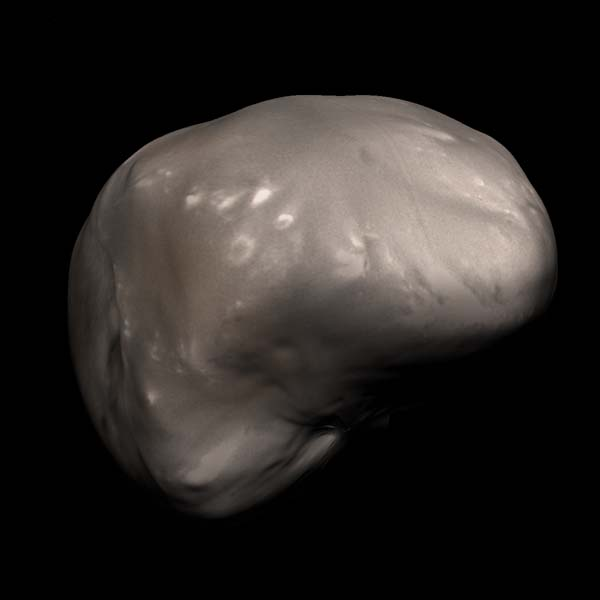
\includegraphics[width=0.285\textwidth, margin=0pt 1ex -20pt 1ex, valign=m]{solsys_deimos.jpg}\\
			\end{tabular}
			}
		\end{tabular}
		}
	& \vfill
	Mars is smaller than Earth (about 1/10 of its mass) with a very thin atmosphere predominantly consisting of carbon dioxide, which nevertheless can produce extensive dust storms that sometimes cover the entire surface. Geological features include Valles Marineris, a 3000 km long network of canyons, and Olympus Mons, the largest shield volcano in the solar system. The polar caps are mainly composed of solid carbon dioxide with small quantities of water ice. Mars has two small irregularly shaped moons, Phobos and Deimos. There have been numerous unmanned missions to Mars, including several rovers to explore the surface.\newline
	\newline
	\textit{The Mars surface textures and elevation data in Orbiter are composed from ESA Mars Express High Resolution Stereo Camera (HRSC) imagery, with missing areas filled from NASA MOC (surface) and MOLA (elevation) data.}\\
	\hline
	\end{tabularx}
\end{table}


\begin{table}[H]
	\begin{tabularx}{\textwidth}{ |lX| }
	\hline\rule{0pt}{2ex}
	\textbf{Vesta} &\\
	\hline\rule{0pt}{2ex}
	\adjustbox{valign=t}{
		\begin{tabular}{ c }
		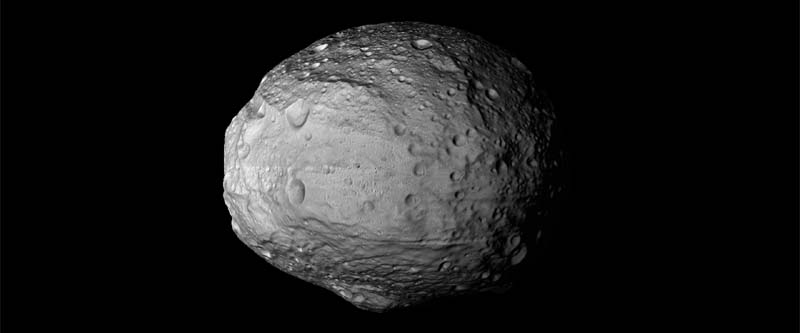
\includegraphics[width=0.6\textwidth, margin=-10pt 1ex -10pt 1ex, valign=m]{solsys_vesta.jpg}\\
		\end{tabular}
		}
	& \vfill
	Vesta is the second-largest asteroid belt object after Ceres. It was visited by the NASA Dawn spacecraft in 2011.\newline
	\newline
	\textit{Surface and elevation data for Orbiter are derived from Dawn HAMO mosaics.}\\
	\hline
	\end{tabularx}
\end{table}


\begin{table}[H]
	\begin{tabularx}{\textwidth}{ |lX| }
	\hline\rule{0pt}{2ex}
	\textbf{Jupiter} &\\
	\hline\rule{0pt}{2ex}
	\adjustbox{valign=t}{
		\begin{tabular}{ c }
		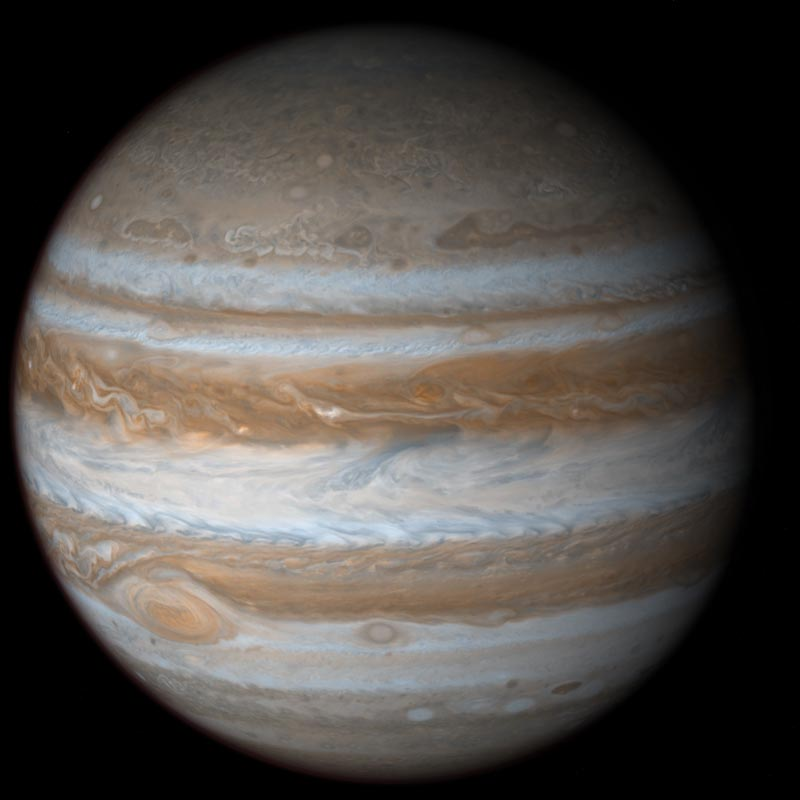
\includegraphics[width=0.6\textwidth, margin=-10pt 1ex -10pt 1ex, valign=m]{solsys_jupiter.jpg}\\
			\adjustbox{valign=t}{
			\begin{tabular}{ ll }
			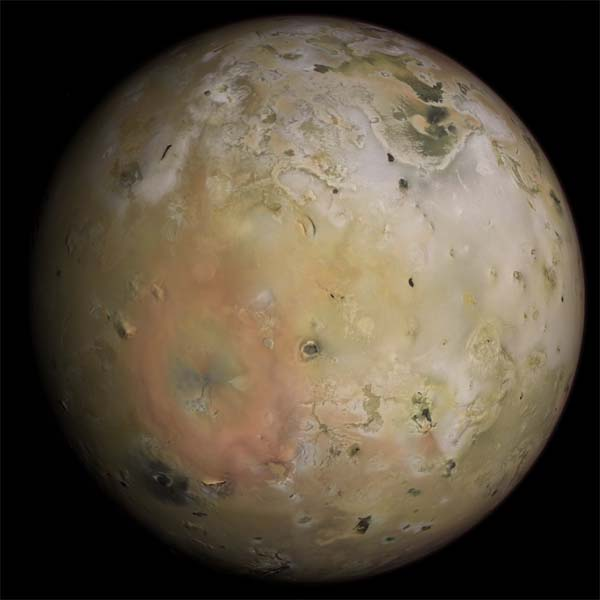
\includegraphics[width=0.285\textwidth, margin=-20pt 1ex 0pt 1ex, valign=m]{solsys_io.jpg} &
			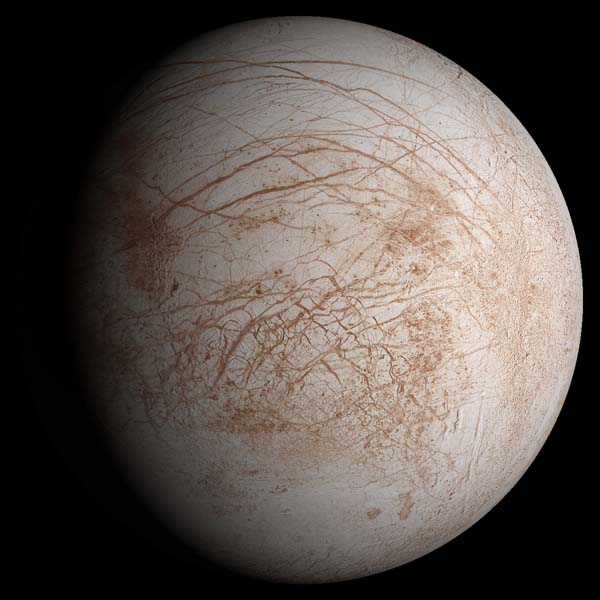
\includegraphics[width=0.285\textwidth, margin=0pt 1ex -20pt 1ex, valign=m]{solsys_europa.jpg}\\
			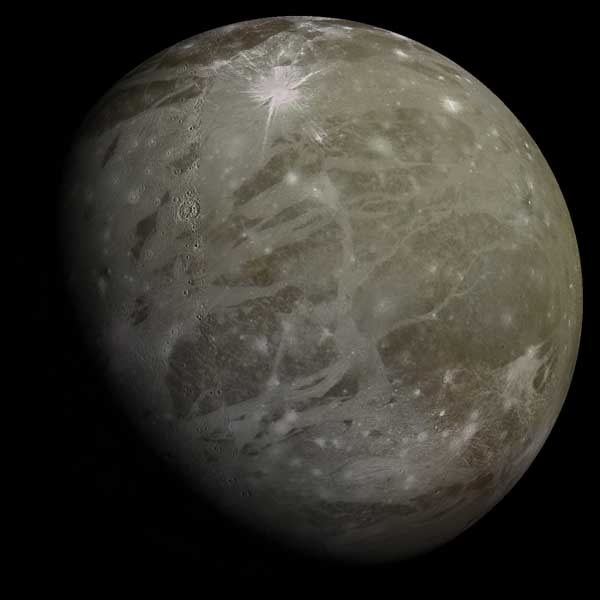
\includegraphics[width=0.285\textwidth, margin=-20pt 1ex 0pt 1ex, valign=m]{solsys_ganymede.jpg} &
			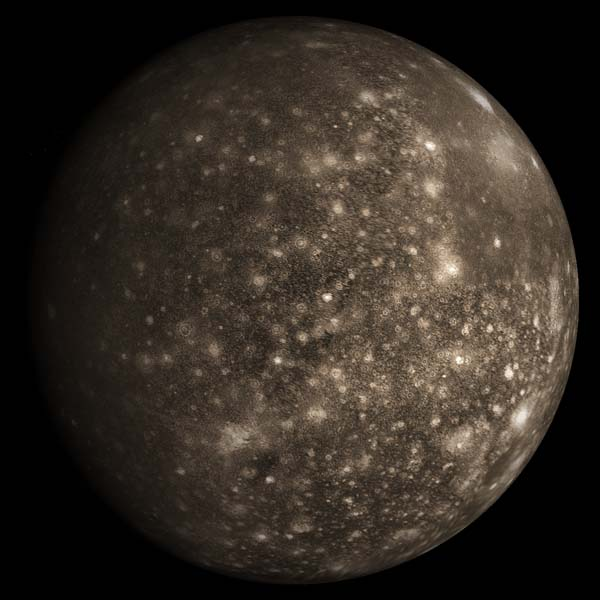
\includegraphics[width=0.285\textwidth, margin=0pt 1ex -20pt 1ex, valign=m]{solsys_callisto.jpg}\\
			\end{tabular}
			}
		\end{tabular}
		}
	& \vfill
	Jupiter is the 5$^{th}$ planet from the Sun, and the innermost of the gas giants. It is the most massive of the planets in the solar system. Its mass allowed it to retain the lighter elements; it is mainly composed of hydrogen and helium, but probably has a core of heavier elements. Jupiter’s atmosphere has a characteristic band structure. Its most prominent feature is the Great Red Spot, an anticyclonic storm that has persisted for centuries.\newline
	Jupiter has a faint ring system and is orbited by at least 80 moons, four of which (the Galilean moons, so called because they were discovered by Galileo Galilei in 1610) are modelled in Orbiter.\newline
	Jupiter and its moons have been visited by several robotic missions, starting with Pioneer 10 and including the Voyager probes, Cassini (en-route to Saturn) and New Horizons.\newline
	\newline
	\textit{In Orbiter, Jupiter visuals are based on Cassini image data (NASA/JPL/Space Science Institute), with cloud maps by Rolf Keibel based on CICLOPS maps.\newline
%TODO move ref?
	The Galilean moon maps are based on Galileo/SSI/Voyager mosaics (Astrogeology Science Center, USGS), with Io elevations based on O. L. White et al., J. Geophys. Res.: Planets 119(6), 1276-1301 (2014)}\\
	\hline
	\end{tabularx}
\end{table}


\begin{table}[H]
	\begin{tabularx}{\textwidth}{ |lX| }
	\hline\rule{0pt}{2ex}
	\textbf{Saturn} &\\
	\hline\rule{0pt}{2ex}
	\adjustbox{valign=t}{
		\begin{tabular}{ c }
		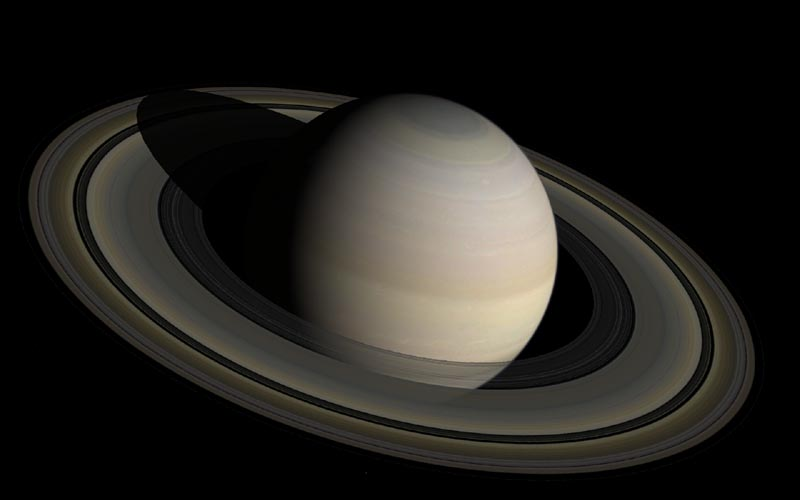
\includegraphics[width=0.6\textwidth, margin=-10pt 1ex -10pt 1ex, valign=m]{solsys_saturn.jpg}\\
			\adjustbox{valign=t}{
			\begin{tabular}{ lll }
			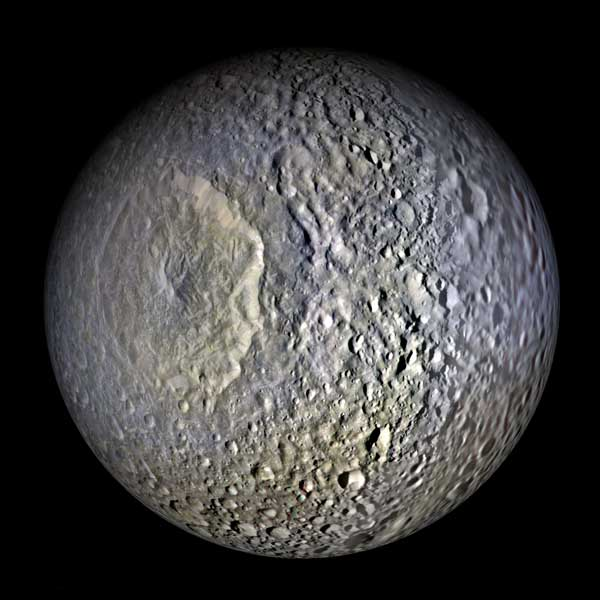
\includegraphics[width=0.18\textwidth, margin=-20pt 1ex 0pt 1ex, valign=m]{solsys_mimas.jpg} &
			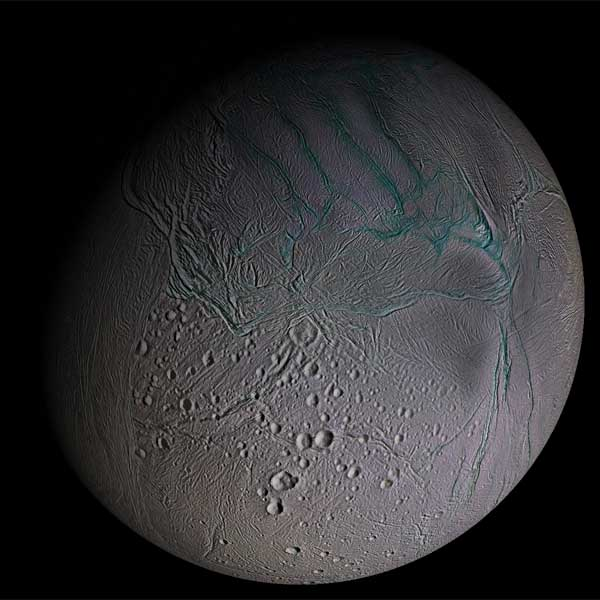
\includegraphics[width=0.18\textwidth, margin=0pt 1ex 0pt 1ex, valign=m]{solsys_enceladus.jpg} &
			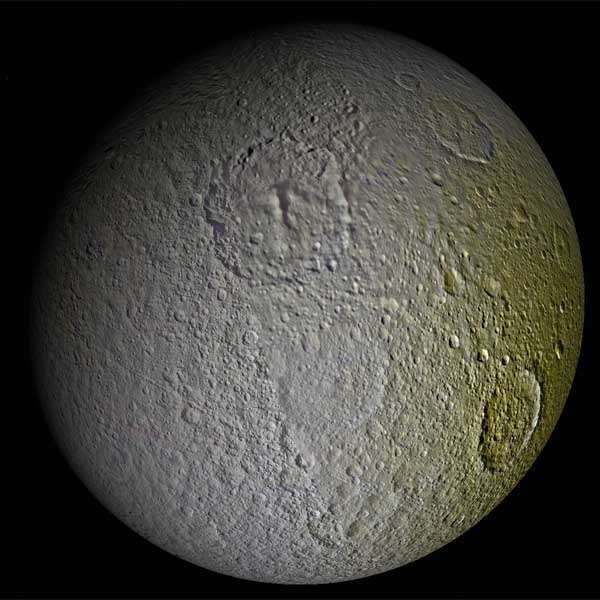
\includegraphics[width=0.18\textwidth, margin=0pt 1ex -20pt 1ex, valign=m]{solsys_tethys.jpg} \\
			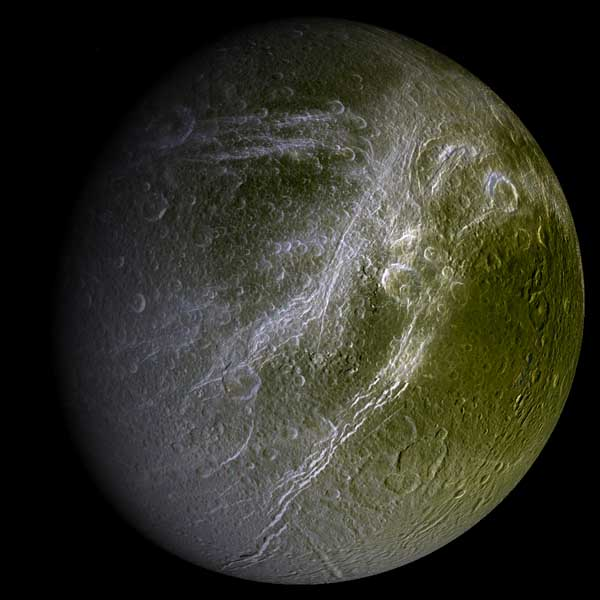
\includegraphics[width=0.18\textwidth, margin=-20pt 1ex 0pt 1ex, valign=m]{solsys_dione.jpg} &
			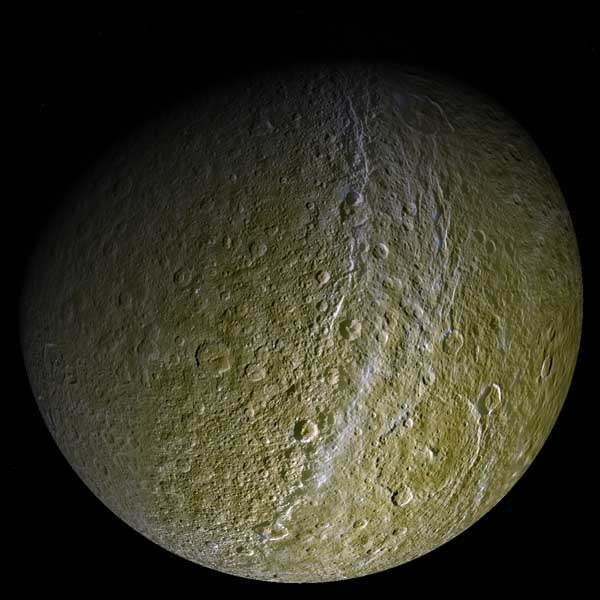
\includegraphics[width=0.18\textwidth, margin=0pt 1ex 0pt 1ex, valign=m]{solsys_rhea.jpg} &
			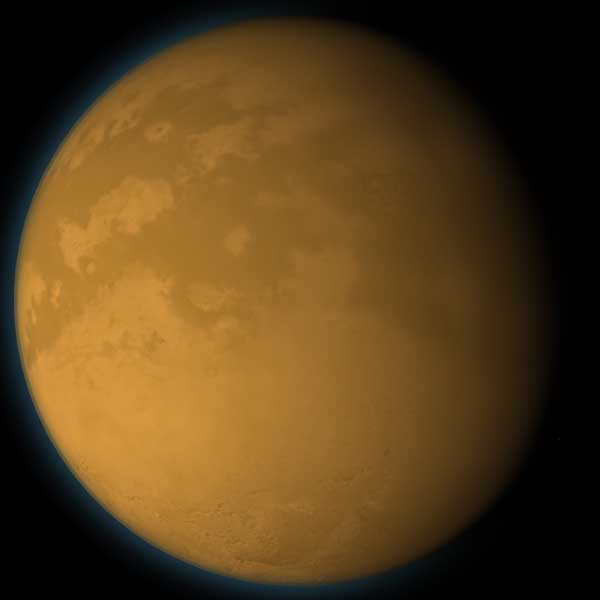
\includegraphics[width=0.18\textwidth, margin=0pt 1ex -20pt 1ex, valign=m]{solsys_titan.jpg}\\
			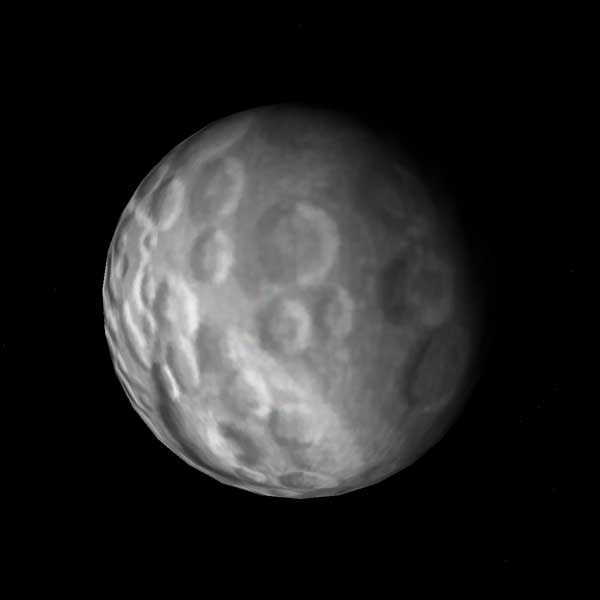
\includegraphics[width=0.18\textwidth, margin=-20pt 1ex 0pt 1ex, valign=m]{solsys_hyperion.jpg} &
			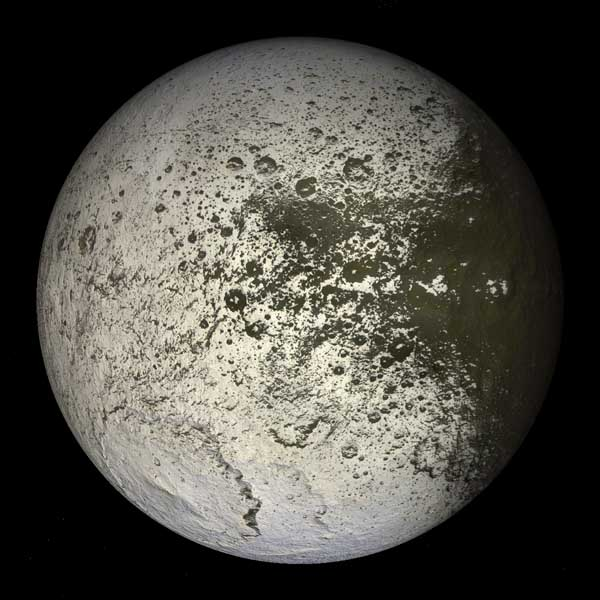
\includegraphics[width=0.18\textwidth, margin=0pt 1ex -20pt 1ex, valign=m]{solsys_iapetus.jpg} &\\
			\end{tabular}
			}
		\end{tabular}
		}
	& \vfill
	Saturn is one of the gas giants and the second-largest planet in the solar system. Like Jupiter, it is composed predominantly of hydrogen and helium. Saturn’s most striking feature is the ring system in the equatorial plane, composed mostly of water ice particles and stretching out from about 1.1 to 3 planet radii, with a thickness of about 20 km.\newline
	Saturn has 83 known moons, not counting a large number of moonlets in the rings. Titan is of comparable size to Mercury and the only moon in the solar system with a substantial atmosphere. There is complex gravitational interaction between the moons and rings, with shepherd moons clearing gaps and keeping rings contained, as well as causing ripples in the ring structure.\newline
	\newline
%TODO move ref?
	\textit{Saturn’s surface and rings in Orbiter are based on maps by Björn Jónsson, adapted by Rolf Keibel. The moon surfaces based on NASA/JPL-Caltech/SSI/Lunar and Planetary Institute, Cassini Central Laboratory for Operations. Titan elevation data P. Corlies et al, Geophysical Research Letters 44(23), 11754-11761 (2017)}\\
	\hline
	\end{tabularx}
\end{table}


\begin{table}[H]
	\begin{tabularx}{\textwidth}{ |lX| }
	\hline\rule{0pt}{2ex}
	\textbf{Uranus} &\\
	\hline\rule{0pt}{2ex}
	\adjustbox{valign=t}{
		\begin{tabular}{ c }
		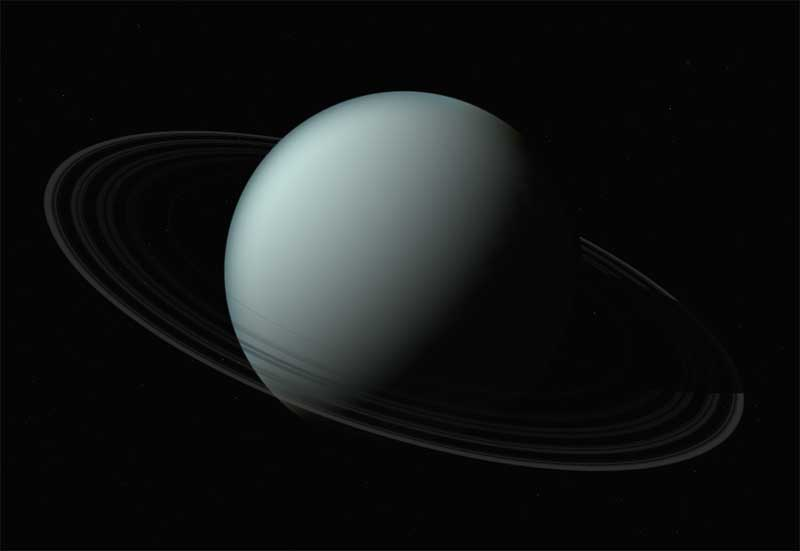
\includegraphics[width=0.6\textwidth, margin=-10pt 1ex -10pt 1ex, valign=m]{solsys_uranus.jpg}\\
			\adjustbox{valign=t}{
			\begin{tabular}{ ll }
			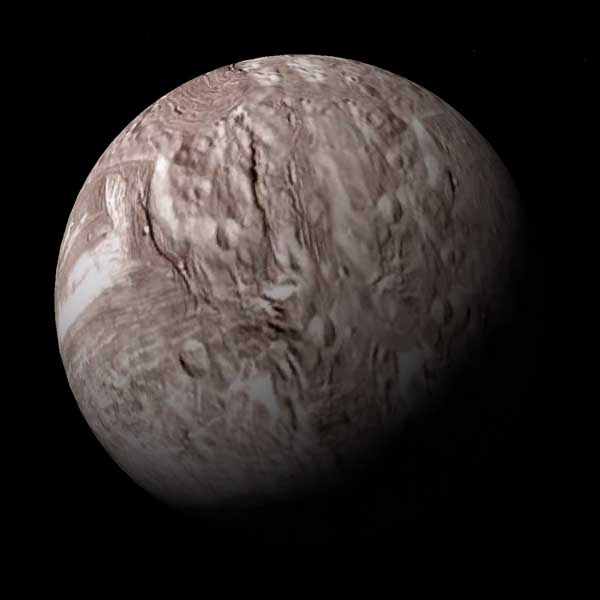
\includegraphics[width=0.285\textwidth, margin=-20pt 1ex 0pt 1ex, valign=m]{solsys_miranda.jpg} &
			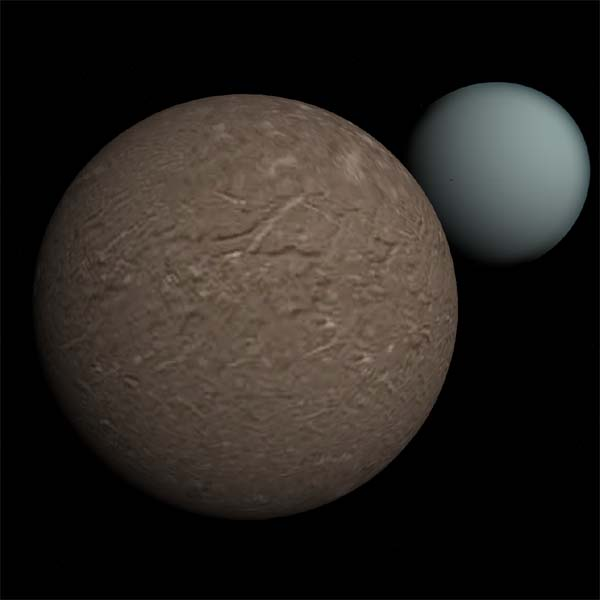
\includegraphics[width=0.285\textwidth, margin=0pt 1ex -20pt 1ex, valign=m]{solsys_ariel.jpg}\\
			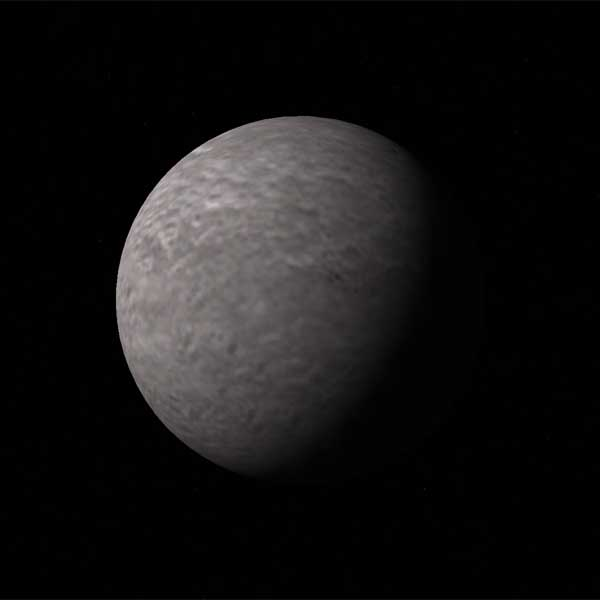
\includegraphics[width=0.285\textwidth, margin=-20pt 1ex 0pt 1ex, valign=m]{solsys_umbriel.jpg} &
			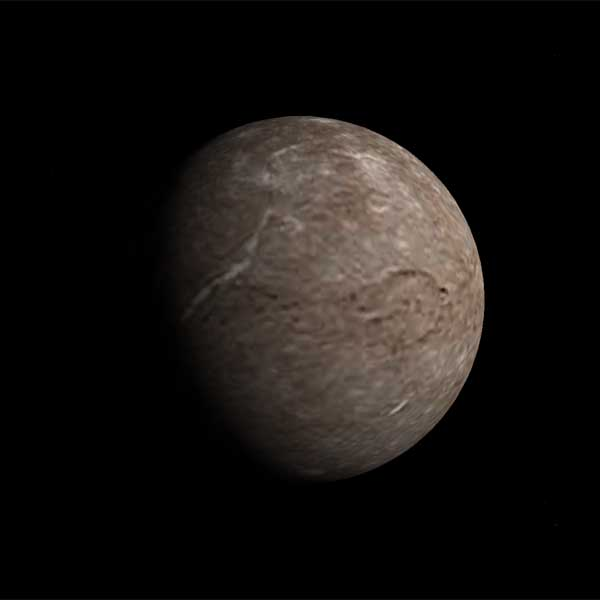
\includegraphics[width=0.285\textwidth, margin=0pt 1ex -20pt 1ex, valign=m]{solsys_titania.jpg}\\
			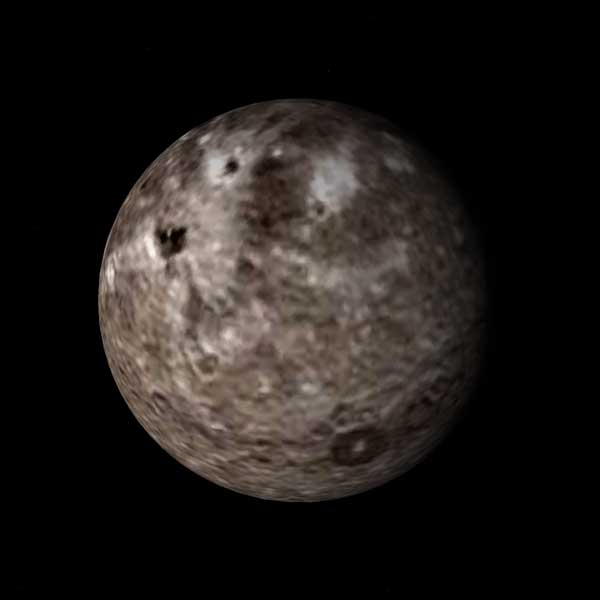
\includegraphics[width=0.285\textwidth, margin=-20pt 1ex 0pt 1ex, valign=m]{solsys_oberon.jpg} &\\
			\end{tabular}
			}
		\end{tabular}
		}
	& \vfill
	Uranus is the seventh planet from the Sun, third-largest by radius and fourth by mass. Its chemical composition is similar to Neptune, containing a solid core of silicate and iron-nickel, a mantle of water/ammonia/methane ice and a hydrogen/helium atmosphere.\newline
	The planet produces little internal heat and emits virtually no excess energy, making it the coldest planet in the solar system.\newline
	Uranus has a ring system consisting of very dark particles and is orbited by at least 27 moons, the main 5 of which are modelled in Orbiter.\newline
	\newline
	\textit{Uranus textures are based on maps by James Hastings-Trew, adapted for Orbiter by Rolf Keibel. The moon textures are based on maps by Robert Stettner and Voyager images adapted by Rolf Keibel.}\\
	\hline
	\end{tabularx}
\end{table}


\begin{table}[H]
	\begin{tabularx}{\textwidth}{ |lX| }
	\hline\rule{0pt}{2ex}
	\textbf{Neptune} &\\
	\hline\rule{0pt}{2ex}
	\adjustbox{valign=t}{
		\begin{tabular}{ c }
		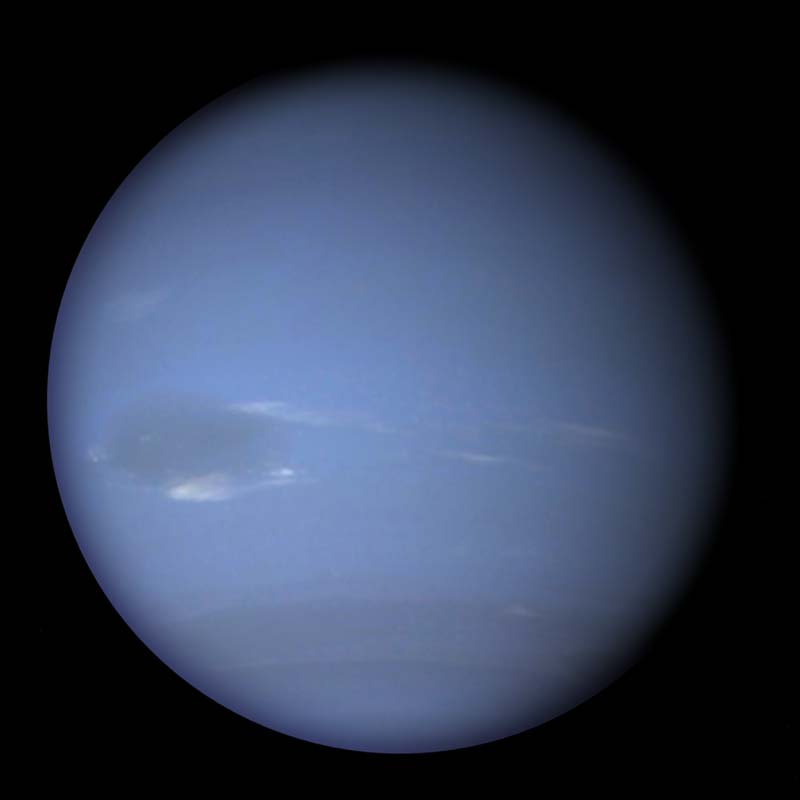
\includegraphics[width=0.6\textwidth, margin=-10pt 1ex -10pt 1ex, valign=m]{solsys_neptune.jpg}\\
			\adjustbox{valign=t}{
			\begin{tabular}{ ll }
			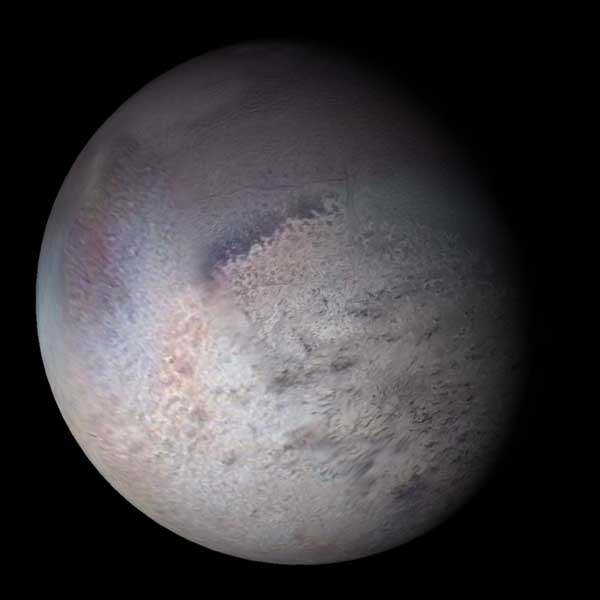
\includegraphics[width=0.285\textwidth, margin=-20pt 1ex 0pt 1ex, valign=m]{solsys_triton.jpg} &
			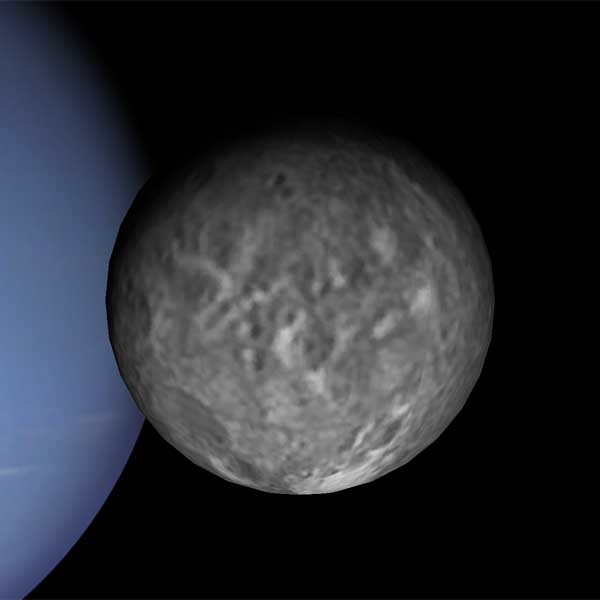
\includegraphics[width=0.285\textwidth, margin=0pt 1ex -20pt 1ex, valign=m]{solsys_proteus.jpg}\\
			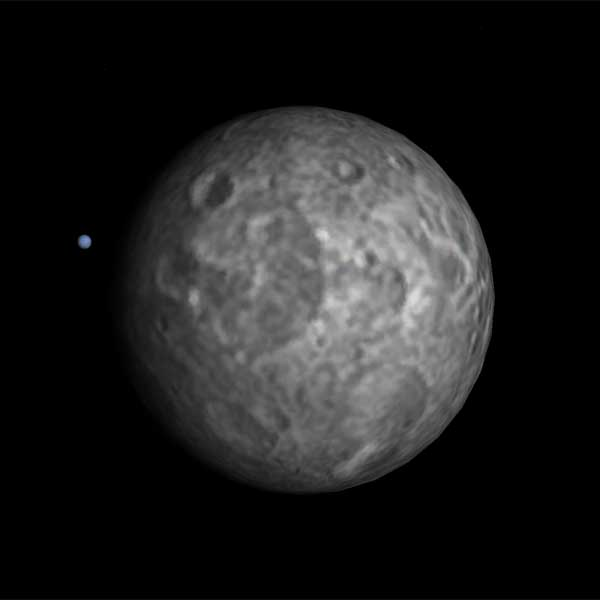
\includegraphics[width=0.285\textwidth, margin=-20pt 1ex 0pt 1ex, valign=m]{solsys_nereid.jpg} &\\
			\end{tabular}
			}
		\end{tabular}
		}
	& \vfill
	Neptune is the farthest planet from the Sun. It is one of the ice giants, and similar in size and composition to Uranus, with a solid rocky core, a mantle of water, ammonia and methane ice, and an atmosphere of hydrogen, helium and methane. The atmosphere frequently features storm systems, visible as dark spots, which can persist for several months and are often accompanied by bright clouds higher up in the atmosphere.\newline
	Neptune has 14 known moons. It also exerts a gravitational influence on the Kuiper belt objects in the region beyond its orbit, including Pluto which orbits in a 2:3 resonance with Neptune.\newline
	\newline
	\textit{Orbiter’s Neptune textures based on a map by James Hastings-Trew, moons by Robert Stettner, from Planetary Mean Orbital Parameters and Moon Maps.}\\
	\hline
	\end{tabularx}
\end{table}

\subsection{Orbital mechanics primer}
Knowing the underlying physics may not be required to fly a spacecraft (after all, you can drive a car without in-depth knowledge of internal combustion - or electromagnetic induction, depending on when you are reading this), but understanding the laws governing the movement of your craft should provide some additional intellectual satisfaction, or (if that doesn’t appeal), may even one day help you get out of an unexpected emergency situation.

\subsubsection{Kepler’s laws of planetary motion}
Johannes Kepler published his three laws of planetary motion in his books \textit{Astronomica Nova} (1609), and \textit{Harmonica Mundi} (1619), refining the Kopernican heliocentric model by dropping the assumption of circular orbits, thereby reconciling the theory with observational data.\\
\\
\textbf{Kepler’s first law:} A planet orbits the Sun in an ellipse, with the Sun at one of the foci.\\
\textbf{Kepler’s second law:} A straight line from the Sun to the planet sweeps out equal areas in equal time intervals.\\
\textbf{Kepler’s third law:} The ratio of the square of a planet’s orbital period with the cube of its semi-major axis is the same for all planets orbiting the Sun.

\subsubsection{Elliptic orbits}
An ellipse is a special case of a conic section (the intersection of the surface of a cone with a plane). The equation of a conic section with the origin in one focus (F) is given in polar coordinates (\textit{r}, \textit{v}) by

\begin{figure}[H]
	\centering
	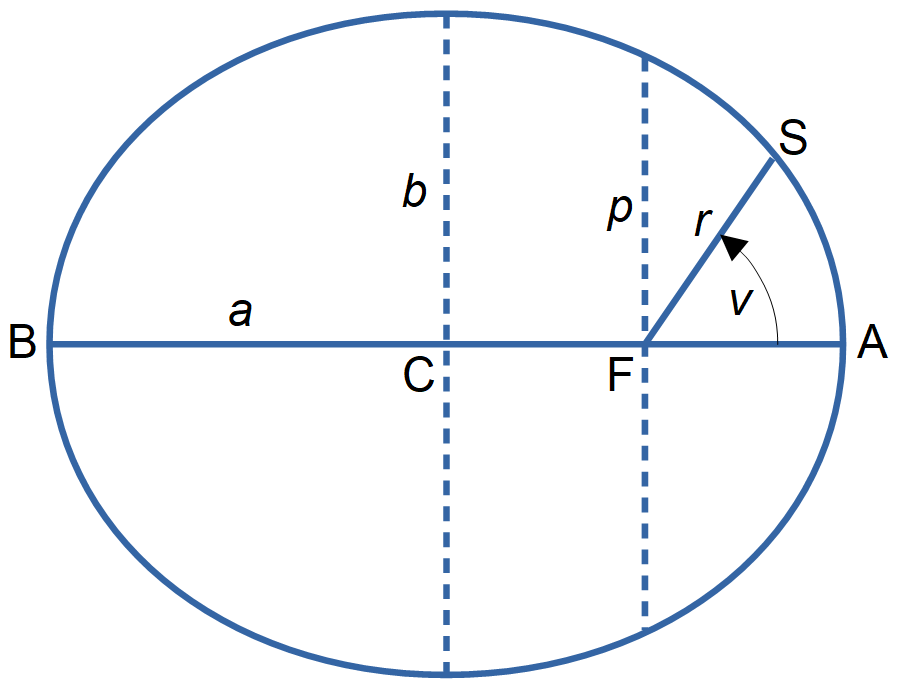
\includegraphics[width=0.5\hsize]{elliptic_orbit.png}
\end{figure}

\[ r = \frac{p}{1 + e \cos v} \]

\noindent
with parameters \textit{e} (eccentricity) and \textit{p} (semi-latus rectum). An ellipse is characterised by eccentricity 0 $\leq$ \textit{e} < 1 (where a circle, e = 0, is taken as the bounding case for an ellipse). The shape of the ellipse is commonly defined by the two parameters \textit{e} and \textit{a} (semi-major axis, the longest semi-diameter), given by

\[ a = \frac{p}{1 - e^{2}} \]

\noindent
Secondary shape parameters can be derived, including the semi-minor axis (shortest semi-diameter) \textit{b}

\[ b = \frac{p}{\sqrt{1 - e^{2}}} = a \sqrt{1 - e^{2}} \]

\noindent
periapsis distance FA (where periapsis A is the point on the ellipse closest to the focus)

\[ r_{pe} = r(v=0) = \frac{p}{1 + e} = (1 - e) a \]

\noindent
and apoapsis distance FB (where apoapsis B is the point on the ellipse farthest from the focus)

\[ r_{ap} = r(v=\pi) = \frac{p}{1 - e} = (1 + e) a \]

\noindent
Kepler’s laws successfully described the motion of celestial bodies in accordance with the observations, but they didn’t provide a reason (the underlying forces) for this motion. This was provided a few decades later by Isaac Newton.

\subsubsection{Newton’s laws of motion}
Newtonian mechanics provides the general framework for describing the motion not only of celestial bodies, but all objects according to their mass (including falling apples). More than three centuries later, Newtonian dynamics is still an appropriate tool for describing the dynamics of a system of bodies for most practical situations (such as those encountered in Orbiter), where the difference to predictions from general relativity (today’s accepted best theory at large scales) are negligible.\\
\\
\textbf{Newton’s first law (law of inertia):} An object on which no external force is acting remains at rest or continues moving at a constant velocity.\\
\textbf{Newton’s second law:} An object experiences an acceleration that is proportional (and in the same direction) as the sum of all forces acting on it, and inversely proportional to its mass.

\[ \textbf{a} = \frac{1}{m} \sum_{i} \textbf{F}_{i} \]

\noindent
\textbf{Newton’s third law:} For every action (force of an object 1 on another object 2) there is an equal and opposite reaction from 2 on 1:

\[ \textbf{F}_{21} = - \textbf{F}_{12} \]

\subsubsection{Newton’s law of gravitation}
Newton introduced the notion of a universal attractive force that works between any two objects. The magnitude of this force is proportional to the object masses $m_{1}$ and $m_{2}$, and inversely proportional to the square of their distance $r_{12}$:

\[ F_{12} = G \frac{m_{1}m_{2}}{r_{12}^{2}} \]

\noindent
where proportionality factor \textit{G} is the \textit{universal gravitational constant}. The direction of the forces is along the straight line from one object to the other:

\[ \textbf{F}_{12} = \hat{\textbf{r}}_{12} F_{12}, \quad \textbf{F}_{21} = - \hat{\textbf{r}}_{12} F_{12} \]

\noindent
where $\hat{\textbf{r}}_{12}$ is the unit vector pointing from object 1 to 2.\\
It is possible to derive Kepler’s laws from Newton’s laws of motion and gravity. This derivation can be found in most textbooks on astrophysics. It requires some calculus (which was developed by Newton for exactly this purpose, in parallel with the work of Gottfried Leibniz). Expressing Kepler’s laws in terms of Newtonian dynamics leads to some useful orbital parameters:\\
The orbital period of an object orbiting a body with mass M is given by

\[ T = \frac{2 \pi}{\sqrt{\mu}} \sqrt{a^{3}} \]

\noindent
with \textit{standard gravitational parameter} $\mu = GM$.\\
The orbital speed \textit{v} as a function of radius \textit{r} is

\[ v = \sqrt{\mu \left(\frac{2}{r} - \frac{1}{a}\right)} \]

\noindent
Maximum and minimum speed occur at periapsis and apoapsis, respectively:

\[ v_{pe} = \sqrt{\frac{(1 + e) \mu}{(1 - e) a}}, \quad v_{ap} = \sqrt{\frac{(1 - e) \mu}{(1 + e) a}} \]

\noindent
and the mean orbital speed is

\[ \bar{v} = \frac{2 \pi a}{T} = \sqrt{\frac{\mu}{a}} = n a \]

\noindent
with \textit{mean angular motion} $n = 2 \pi / T$.\\
The \textit{specific orbital energy} (or vis-viva energy) \textit{E} is the sum of potential energy $E_{p}$ and kinetic energy $E_{k}$ of an orbiting body. \textit{E} is constant along the orbit.

\[ E = E_{k} + E_{p} = \frac{v^{2}}{2} - \frac{\mu}{r} = - \frac{1}{2} \frac{\mu^{2}}{h^{2}}(1 - e^{2}) \]

\noindent
where \textit{h} is the specific angular momentum of the orbiting body. For specific types of orbit, \textit{E} is given by

\[ E =
\left\{
\begin{array}{ll}
	-\frac{\mu}{2a} & e < 1 \\
	0 & e = 1 \\
	\frac{\mu}{2a} & e > 1 \\
\end{array} 
\right. \]

\subsubsection{Orbital elements}
The orbit of an object around a central body is completely defined by a set of 6 scalar parameters. In addition to the two parameters \textit{a} and \textit{e} discussed above that describe the shape of the ellipse, a further parameter $\omega$ (argument of periapsis) defines the rotation angle of the ellipse in the orbital plane. Two parameters \textit{i} (inclination) and $\Omega$ (longitude of the ascending node) define the orientation of the orbital plane in space relative to a reference coordinate system (e.g. plane of the ecliptic with vernal point {\Aries} as reference direction), and a final parameter \textit{v(t)} (true anomaly) at epoch defines the angular position of the orbiting object along the orbit at a specific time \textit{t}. These are the Keplerian or 2-body elements of an unperturbed orbit. Equivalently, the orbit can also be defined by the \textit{state vectors} of the orbiting object at a given time: position \textbf{r}(t) and velocity \textbf{v}(t). It is possible to calculate the orbital elements from the state vectors and vice versa.

\begin{figure}[H]
	\centering
	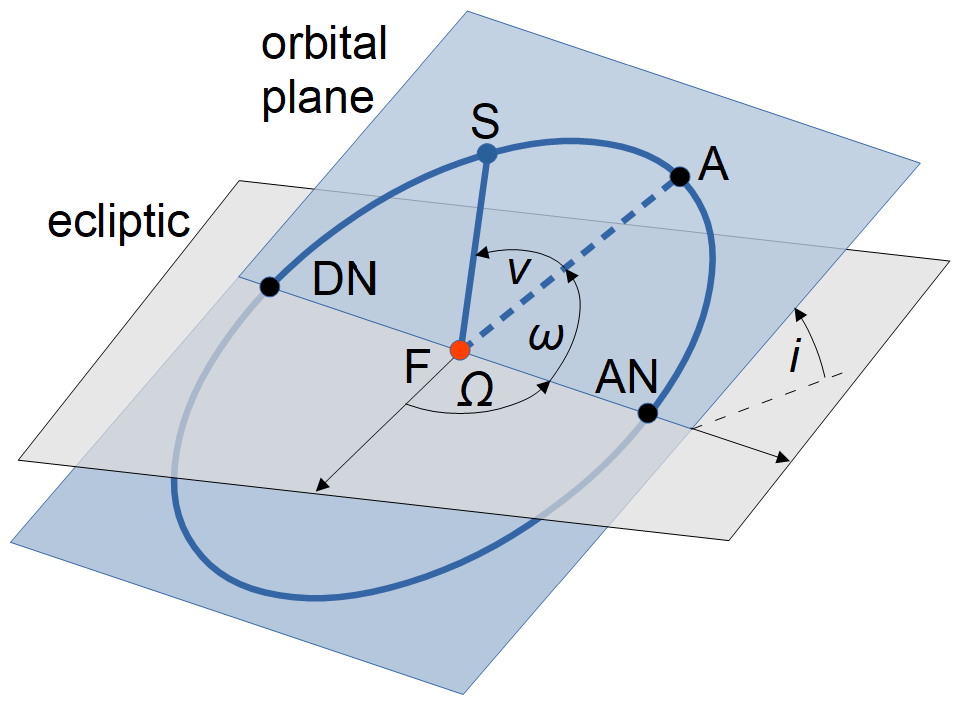
\includegraphics[width=0.5\hsize]{orbital_elements.png}
\end{figure}

\noindent
From Newtonian dynamics we know that Kepler’s laws strictly apply only to two-body problems. In the solar system containing multiple bodies which all exert a gravitational force on each other, all orbits are perturbed to some extent from the elliptical shape. In some cases these perturbations are small, but often they cannot be neglected. For example, the Earth’s orbit around the Sun is significantly affected by the gravitational influence of its relatively large moon. In this case, it is more appropriate to describe the trajectory the \textit{barycentre} (the centre of mass) of the Earth-Moon system around the Sun as a two-body problem, and the orbits of Earth and Moon around each other as a separate two-body problem on top of it. If even more precision is required, e.g. to factor in the gravitational influence of other planets, an n-body treatment is required, which can generally only be solved numerically.\\
In perturbed orbits, the orbital elements change over time. Computing the 2-body elements from the state vectors at a specific time $t_{0}$ results in the expression of an orbit that the orbiting object would follow in the absence of perturbing influences (osculating orbit). The elements are the \textit{osculating elements} at $t_{0}$.

\subsubsection{Kepler’s equation}
Computing the true anomaly \textit{v} is not trivial for eccentric orbits, because the orbital velocity is changing along the orbit according to Kepler’s second law. It is sometimes useful to substitute v with the \textit{mean anomaly M}, a parameter that is changing linearly with time:

\[ M(t) = n(t - t_{0}) \]

\noindent
where $t_{0}$ is the time of periapsis passage. M is the angular position of a body in a circular orbit with the same semi-major axis \textit{a} (and thus the same orbital period \textit{T}) and the same periapsis passage time $t_{0}$.

\begin{figure}[H]
	\centering
	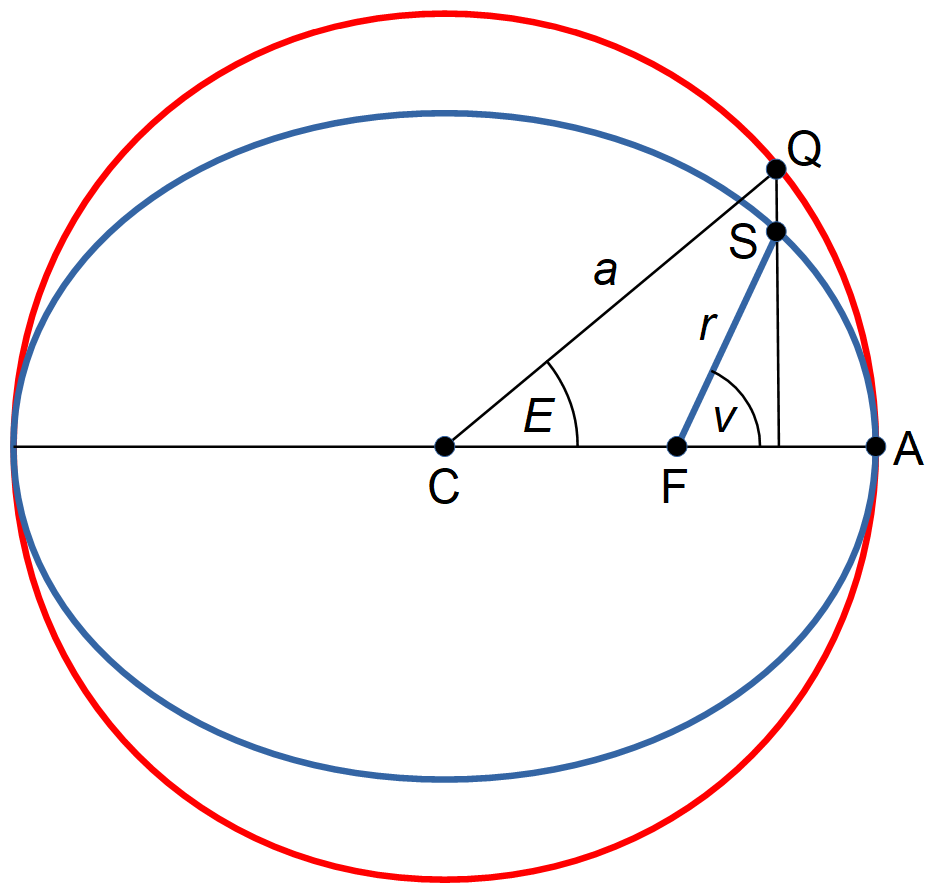
\includegraphics[width=0.5\hsize]{mean_anomaly.png}
\end{figure}

\noindent
To compute true anomaly from mean anomaly, we first introduce the \textit{eccentric anomaly E}: Define a circle with radius \textit{a} whose centre coincides with the centre of the elliptic orbit. Project the object position S perpendicular to the semi-major axis onto the circle (Q). Then \textit{E} is defined as the angle ACQ between periapsis A and Q, measured at the centre C of the circle.\\
The relationship between orbit radius \textit{r} and \textit{E} is given by

\[ r = a (1 - e \cos E) \]

\noindent
\textit{v} can be computed from \textit{E} by

\[ \tan \frac{v}{2} = \sqrt{\frac{1 + e}{1 - e}} \tan \frac{E}{2} \]

\noindent
and \textit{E} is related to \textit{M} via Kepler’s equation

\[ E(t) - e \sin E(t) = M(t) \]

\noindent
which cannot be solved in closed form, but generally requires an iterative solution.

\subsubsection{Sphere of influence and patched conic approximation}
Planning the trajectory of an interplanetary space probe requires the solution of a multi-body problem that takes into account the gravitational influence of Earth, the Sun and the target planet(s) and possibly their moons. This usually involves a numerical simulation that propagates the flight path in time, given a set of initial conditions and potential mid-flight manoeuvres. Such a solution can be computationally expensive, in particular if many trajectory simulations are required, for example to find suitable launch parameters for a trip that involves multiple planet encounters and gravity assist manoeuvres.

\begin{figure}[H]
	\centering
	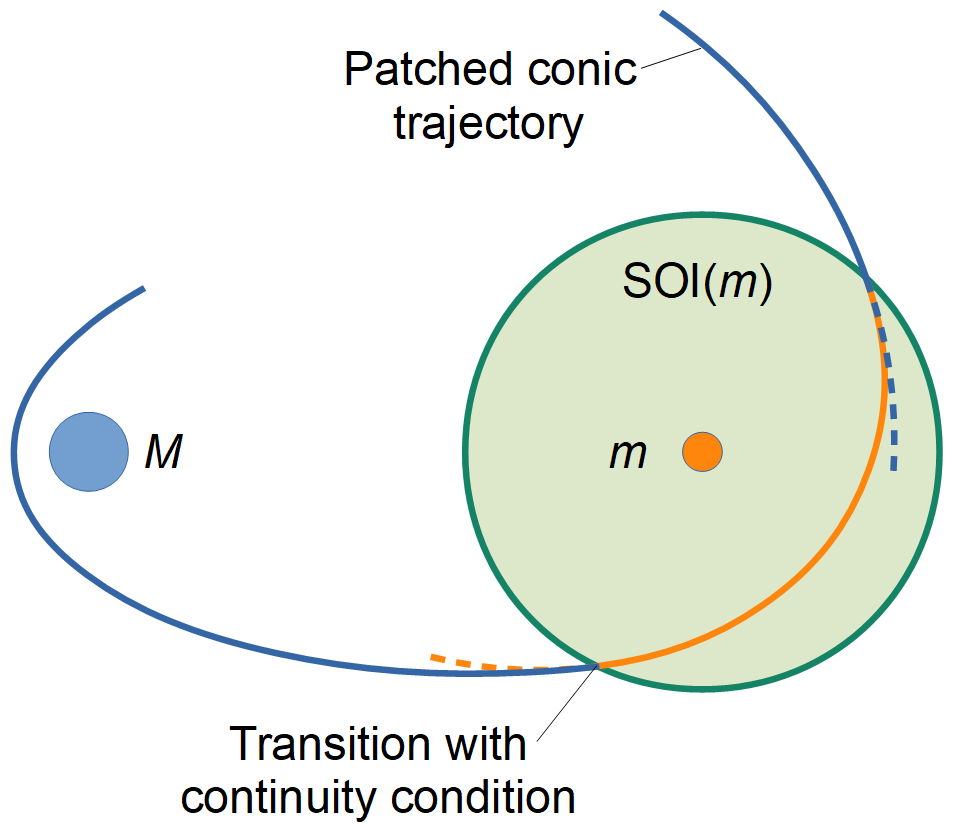
\includegraphics[width=0.5\hsize]{soi.png}
\end{figure}

\noindent
An alternative to the full multi-body solution is the \textit{patched conic approximation}. Given two gravitational sources with masses \textit{M} and \textit{m}, the less massive body \textit{m} is assigned a \textit{sphere of influence}, in the simplest form defined as a sphere with radius

\[ r_{SOI} = a \left( \frac{m}{M} \right)^{2/5} \]

\noindent
where \textit{a} is the semi-major axis of the orbit of \textit{m} around \textit{M}. The region of influence of \textit{M} is all space outside the smaller body’s SOI.\\
The spacecraft on a point along its trajectory is assumed to be under the gravitational influence of only the single body whose SOI is currently traversed. As soon as the SOI boundary of another body is crossed, that body’s gravitational field is exclusively used for the computation of the next part of the trajectory, subject to the boundary condition that the state vectors (position \textbf{r} and velocity \textbf{v}) are continuous across the SOI boundary.\\
In the solar system, SOI can be assigned for each planet or other body orbiting the Sun. On a second level, a planet’s moons may be assigned their own SOI that are embedded in the planet’s SOI.\\
The patched conic method is not exact - in particular at the SOI boundaries, where the gravitational influences of the two bodies are approximately equal, neglecting one of them may lead to errors in the trajectory prediction. However, it can be a reasonable initial estimate for designing a mission, and can be refined by a precise numerical multi-body simulation if required.


\subsection{Selected constants and parameters}
These data may be useful when planning missions across the solar system.

\subsubsection{Astrodynamic constants}

%\begin{table}[H]
	%\centering
	\begin{longtable}{ |p{0.35\textwidth}|p{0.14\textwidth}|p{0.42\textwidth}| }
	\hline\rule{0pt}{2ex}
	\textbf{Constant} & \textbf{Symbol} & \textbf{Value}\\
	\hline\rule{0pt}{2ex}
	Julian day & d & 86400 s\\
	\hline\rule{0pt}{2ex}
	Julian year & yr & 365.25 d\\
	\hline\rule{0pt}{2ex}
	Julian century & Cy & 36525 d\\
	\hline\rule{0pt}{2ex}
	Speed of light & c & 299792458 m/s\\
	\hline\rule{0pt}{2ex}
	Gaussian gravitational constant & k & 0.01720209895 (AU$^{3}$/d$^{2}$)$^{1/2}$\\
	\hline
	\caption{Defining constants}
	\end{longtable}
%\end{table}

%TODO add vesta, ceres, etc
%\begin{table}[H]
	%\centering
	\begin{longtable}{ |p{0.35\textwidth}|p{0.14\textwidth}|p{0.42\textwidth}| }
	\hline\rule{0pt}{2ex}
	\textbf{Constant} & \textbf{Symbol} & \textbf{Value}\\
	\hline\rule{0pt}{2ex}
	Mean sidereal day & & 86164.09054 s = 23:56:04.09054\\
	\hline\rule{0pt}{2ex}
	Sidereal year (quasar ref. frame) & & 365.25636 d\\
	\hline\rule{0pt}{2ex}
	Light time for 1 AU & $\tau_{A}$ & 499.004783806 ($\pm$ 0.00000001) s\\
	\hline\rule{0pt}{2ex}
	Gravitational constant & G & 6.67259 ($\pm$ 0.00030) $\times$ 10$^{-11}$ kg$^{-1}$ m$^{3}$ s$^{-2}$\\
	\hline\rule{0pt}{2ex}
	General precession in longitude & & 5028.83 ($\pm$ 0.04) arcsec/Cy\\
	\hline\rule{0pt}{2ex}
	Obliquity of ecliptic (J2000.0) & $\epsilon$ & 84381.412 ($\pm$ 0.005) arcsec\\
	\hline\rule{0pt}{2ex}
	Mass: Sun / Mercury & & 6023600. ($\pm$ 250.)\\
	\hline\rule{0pt}{2ex}
	Mass: Sun / Venus & & 408523.71 ($\pm$ 0.06)\\
	\hline\rule{0pt}{2ex}
	Mass: Sun / (Earth + Moon) & & 328900.56 ($\pm$ 0.02)\\
	\hline\rule{0pt}{2ex}
	Mass: Sun / (Mars system) & & 3098708. ($\pm$ 9.)\\
	\hline\rule{0pt}{2ex}
	Mass: Sun / (Jupiter system) & & 1047.3486 ($\pm$ 0.0008)\\
	\hline\rule{0pt}{2ex}
	Mass: Sun / (Saturn system) & & 3497.898 ($\pm$ 0.018)\\
	\hline\rule{0pt}{2ex}
	Mass: Sun / (Uranus system) & & 22902.98 ($\pm$ 0.03)\\
	\hline\rule{0pt}{2ex}
	Mass: Sun / (Neptune system) & & 19412.24 ($\pm$ 0.04)\\
	\hline\rule{0pt}{2ex}
	Mass: Sun / (Pluto system) & & 1.35 ($\pm$ 0.07) $\times$ 10$^{8}$\\
	\hline\rule{0pt}{2ex}
	Mass: Moon / Earth & & 0.012300034 ($\pm$ 3 $\times$ 10$^{-9}$)\\
	\hline
	\caption{Primary constants}
	\end{longtable}
%\end{table}

%\begin{table}[H]
	%\centering
	\begin{longtable}{ |p{0.35\textwidth}|p{0.14\textwidth}|p{0.42\textwidth}| }
	\hline\rule{0pt}{2ex}
	\textbf{Constant} & \textbf{Symbol} & \textbf{Value}\\
	\hline\rule{0pt}{2ex}
	Astronomical unit distance & c $\times$ $\tau_{A}$ = AU & 1.49597870691 $\times$ 10$^{11}$ ($\pm$ 3) m\\
	\hline\rule{0pt}{2ex}
	Heliocentric gravitational constant & k$^{2}$ AU$^{3}$ d$^{-2}$ = GM$_{SUN}$ & 1.32712440018 $\times$ 10$^{20}$ ($\pm$ 8 $\times$ 10$^{9}$) m$^{3}$ s$^{-2}$\\
	\hline\rule{0pt}{2ex}
	Mass: Earth / Moon & & 81.30059 ($\pm$ 0.00001)\\
	\hline
	\caption{Derived constants}
	\end{longtable}
%\end{table}

\noindent
All values from \cite{standish1995}\\
\\
\underline{Notes:}\\
Data are from the 1994 IAU file of current best estimates. Planetary ranging determines the Earth/Moon mass ratio. The value for 1 AU is taken from JPL’s current planetary ephemeris DE-405.\\
\\
\textbf{Planetary mean orbital elements and centennial rates}

%TODO add vesta, ceres, etc
%\begin{table}[H]
	%\centering
	\begin{longtable}{ |p{0.1\textwidth}|p{0.13\textwidth}|p{0.13\textwidth}|p{0.1\textwidth}|p{0.12\textwidth}|p{0.11\textwidth}|p{0.11\textwidth}| }
	\hline\rule{0pt}{2ex}
	\textbf{Planet} & \textbf{a [AU]} & \textbf{e} & \textbf{i [deg]} & \textbf{$\Omega$ [deg]} & \textbf{$\bar{\omega}$ [deg]} & \textbf{L [deg]}\\
	\hline\rule{0pt}{2ex}
	Mercury & 0.38709893 & 0.20563069 & 7.00487 & 48.33167 & 77.45645 & 252.25084\\
	\hline\rule{0pt}{2ex}
	Venus & 0.72333199 & 0.00677323 & 3.39471 & 76.68069 & 131.53298 & 181.97973\\
	\hline\rule{0pt}{2ex}
	Earth & 1.00000011 & 0.01671022 & 0.00005 & -11.26064 & 102.94719 & 100.46435\\
	\hline\rule{0pt}{2ex}
	Mars & 1.52366231 & 0.09341233 & 1.85061 & 49.57854 & 336.04084 & 355.45332\\
	\hline\rule{0pt}{2ex}
	Jupiter & 5.20336301 & 0.04839266 & 1.30530 & 100.55615 & 14.75385 & 34.40438\\
	\hline\rule{0pt}{2ex}
	Saturn & 9.53707032 & 0.05415060 & 2.48446 & 113.71504 & 92.43194 & 49.94432\\
	\hline\rule{0pt}{2ex}
	Uranus & 19.19126393 & 0.04716771 & 0.76986 & 74.22988 & 170.96424 & 313.23218\\
	\hline\rule{0pt}{2ex}
	Neptune & 30.06896348 & 0.00858587 & 1.76917 & 131.72169 & 44.97135 & 304.88003\\
	\hline\rule{0pt}{2ex}
	Pluto & 39.48168677 & 0.24880766 & 17.14175 & 110.30347 & 224.06676 & 238.92881\\
	\hline
	\end{longtable}
%\end{table}

%TODO add vesta, ceres, etc
%\begin{table}[H]
	%\centering
	\begin{longtable}{ |p{0.1\textwidth}|p{0.13\textwidth}|p{0.13\textwidth}|p{0.08\textwidth}|p{0.11\textwidth}|p{0.1\textwidth}|p{0.15\textwidth}| }
	\hline\rule{0pt}{2ex}
	\textbf{Planet} & \textbf{da/dt [AU/Cy]} & \textbf{de/dt [/Cy]} & \textbf{di/dt [''/Cy]} & \textbf{d$\Omega$/dt [''/Cy]} & \textbf{d$\bar{\omega}$/dt [''/Cy]} & \textbf{dL/dt [''/Cy]}\\
	\hline\rule{0pt}{2ex}
	Mercury & 0.00000066 & 0.00002527 & -23.51 & -446.30 & 573.57 & 538101628.29\\
	\hline\rule{0pt}{2ex}
	Venus & 0.00000092 & -0.00004938 & -2.86 & -996.89 & -108.80 & 210664136.06\\
	\hline\rule{0pt}{2ex}
	Earth & -0.00000005 & -0.00003804 & -46.94 & -18228.25 & 1198.28 & 129597740.63\\
	\hline\rule{0pt}{2ex}
	Mars & -0.00007221 & 0.00011902 & -25.47 & -1020.19 & 1560.78 & 68905103.78\\
	\hline\rule{0pt}{2ex}
	Jupiter & 0.00060737 & -0.00012880 & -4.15 & 1217.17 & 839.93 & 10925078.35 \\
	\hline\rule{0pt}{2ex}
	Saturn & -0.00301530 & -0.00036762 & 6.11 & -1591.05 & -1948.89 & 4401052.95\\
	\hline\rule{0pt}{2ex}
	Uranus & 0.00152025 & -0.00019150 & -2.09 & -1681.40 & 1312.56 & 1542547.79\\
	\hline\rule{0pt}{2ex}
	Neptune & -0.00125196 & 0.0000251 & -3.64 & -151.25 & -844.43 & 786449.21\\
	\hline\rule{0pt}{2ex}
	Pluto & -0.00076912 & 0.00006465 & 11.07 & -37.33 & -132.25 & 522747.90\\
	\hline
	\end{longtable}
%\end{table}

\noindent
a: semi-major axis, e: eccentricity, i: inclination, $\Omega$: longitude of the ascending node, $\bar{\omega}$: longitude of perihelion, L: mean longitude, Cy: Julian century, '': arcsec\\
Epoch = J2000 = 2000 January 1.5\\
All values from \cite{seidelmann1992p316}\\
\\
\underline{Notes:}\\
The tables contain mean orbit solutions from a 250 yr. least squares fit of the DE 200 planetary ephemeris to a Keplerian orbit where each element is allowed to vary linearly with time. This solution fits the terrestrial planet orbits to $\sim$25'' or better, but achieves only $\sim$600'' for Saturn. Elements are referenced to mean ecliptic and equinox of J2000 at the J2000 epoch (2451545.0 JD).

\subsubsection{Selected physical parameters}

%TODO add vesta, ceres, etc
%\begin{table}[H]
	%\centering
	\begin{longtable}{ |p{0.1\textwidth}|p{0.16\textwidth}|p{0.15\textwidth}|p{0.17\textwidth}|p{0.13\textwidth}|p{0.12\textwidth}| }
	\hline\rule{0pt}{2ex}
	\textbf{Planet} & \textbf{mean radius [km]} & \textbf{mass [10$^{23}$ km]} & \textbf{density [g/cm$^{3}$]} & \textbf{sidereal rotation period [h]} & \textbf{sidereal orbit period [yr]}\\
	\hline\rule{0pt}{2ex}
	Mercury & 2440. $\pm$ 1. & 3.301880 & 5.427 & 1407.509 & 0.2408445\\
	\hline\rule{0pt}{2ex}
	Venus & 6051.84 $\pm$ 0.01 & 48.6855374 & 5.204 & -5832.444 & 0.6151826\\
	\hline\rule{0pt}{2ex}
	Earth & 6371.01 $\pm$ 0.02 & 59.73698968 & 5.515 & 23.93419** & 0.9999786\\
	\hline\rule{0pt}{2ex}
	Mars & 3389.92 $\pm$ 0.04 & 6.418542 & 3.9335 $\pm$ 0.0004 & 24.622962 & 1.88071105\\
	\hline\rule{0pt}{2ex}
	Jupiter & 69911. $\pm$ 6. & 18986.111 & 1.326 & 9.92425 & 11.856523\\
	\hline\rule{0pt}{2ex}
	Saturn & 58232. $\pm$ 6. & 5684.6272 & 0.6873 & 10.65622 & 29.423519\\
	\hline\rule{0pt}{2ex}
	Uranus & 25362. $\pm$ 12. & 868.32054 & 1.318 & 17.24 $\pm$ 0.01 & 83.747407\\
	\hline\rule{0pt}{2ex}
	Neptune & 24624. $\pm$ 21. & 1024.569 & 1.638 & 16.11 $\pm$ 0.01 & 163.72321\\
	\hline\rule{0pt}{2ex}
	Pluto* & 1151 & 0.15 & 1.1 & 153.28 & 248.0208\\
	\hline
	\end{longtable}
%\end{table}

%TODO add vesta, ceres, etc
%\begin{table}[H]
	%\centering
	\begin{longtable}{ |p{0.1\textwidth}|p{0.17\textwidth}|p{0.17\textwidth}|p{0.21\textwidth}|p{0.21\textwidth}| }
	\hline\rule{0pt}{2ex}
	\textbf{Planet} & \textbf{V(1,0) [mag.]} & \textbf{Geometric albedo} & \textbf{Equatorial gravity [m/s$^{2}$]} & \textbf{Escape velocity [km/s]}\\
	\hline\rule{0pt}{2ex}
	Mercury & -0.42 & 0.106 & 3.701 & 4.435\\
	\hline\rule{0pt}{2ex}
	Venus & -4.4 & 0.65 & 8.87 & 10.361\\
	\hline\rule{0pt}{2ex}
	Earth & -3.86 & 0.367 & 9.780327 & 11.186\\
	\hline\rule{0pt}{2ex}
	Mars & -1.52 & 0.15 & 3.69 & 5.027\\
	\hline\rule{0pt}{2ex}
	Jupiter & -9.4 & 0.52 & 23.12 $\pm$ 0.01 & 59.5\\
	\hline\rule{0pt}{2ex}
	Saturn & -8.88 & 0.47 & 8.96 $\pm$ 0.01 & 35.5\\
	\hline\rule{0pt}{2ex}
	Uranus & -7.19 & 0.51 & 8.69 $\pm$ 0.01 & 21.3\\
	\hline\rule{0pt}{2ex}
	Neptune & -6.87 & 0.41 & 11.00 $\pm$ 0.05 & 23.5\\ 
	\hline\rule{0pt}{2ex}
	Pluto* & -1.0* & 0.3* & 0.655 & 1.3\\
	\hline
	\end{longtable}
%\end{table}

\noindent
All values from \cite{yoder1995} except Pluto data from \cite{seidelmann1992p706}. Mercury to Neptune masses derived from standard gravitational parameter (GM) data in \cite{yoder1995}.\\
** Orbiter uses 23.93447 h (=23 h 56 m 4.09 s) which gives better long-term stability.

\end{document}
